% ======================================================================
% 基于迭代Leiden聚类与大模型增强评估的层次化新闻主题编目
% ======================================================================
\documentclass[10pt,twocolumn,twoside]{ctexart}

\usepackage{amsmath,amssymb,amsfonts}
\usepackage{graphicx}
\usepackage{booktabs}
\usepackage[top=2.2cm,bottom=2.2cm,left=1.6cm,right=1.6cm]{geometry}
\usepackage{hyperref}
\usepackage{natbib}
\usepackage{algorithm}
\usepackage{algpseudocode}
\usepackage{caption}
\usepackage{subcaption}
\usepackage{xcolor}
\usepackage{enumitem}
\usepackage{tabularx}
\usepackage{multirow}
\usepackage{adjustbox}
\usepackage{tikz}
\usetikzlibrary{positioning, arrows.meta, shapes.geometric, fit, backgrounds, calc}

% 中文字体设置
\setCJKmainfont{Songti SC}
\setCJKsansfont{Heiti SC}
\setCJKmonofont{STHeiti}

% Colors
\definecolor{primary}{HTML}{1f5878}
\definecolor{secondary}{HTML}{2c6e8a}
\definecolor{accent}{HTML}{4a9bb5}
\definecolor{orange}{HTML}{e67e22}
\definecolor{green}{HTML}{27ae60}
\definecolor{lightgray}{HTML}{f5f5f5}

\hypersetup{colorlinks=true,linkcolor=primary,citecolor=primary,urlcolor=secondary}

\title{\textbf{基于图划分与大模型自监督的\\层次化新闻编目方法}}

\author{匿名作者\thanks{课程作业}\\\texttt{\{anonymous\}@submission.org}}

\date{}

\begin{document}
\maketitle

\begin{abstract}
本文提出了一套无监督与自监督相结合的新闻标题编目流水线，通过13组实验覆盖四个设计维度
（嵌入策略、聚类范式、离群点处理、大模型集成）。系统融合了$k$-近邻图构建、
Leiden社区发现、六规则评分器与大模型增强评估（MiniMax-M2.7），
由有限状态机统一编排。大模型生成的主题质量等级（A/B/C/D）在自监督精炼循环中充当
伪标签，而基于深度的自训练机制则将API成本降低60\%。该流水线实现了\textbf{94.3\%的覆盖率}，
产出\textbf{585个层次化组织的叶子主题}且\textbf{零离群点}——较BERTopic（34.2\%离群率）
有显著提升。我们在4项指标上对5种聚类范式进行了基准对比，并证明将无监督图划分
与自监督大模型评估交替执行，能够生成比任一范式单独使用更具可解释性的层次化分类体系。
代码：\url{https://github.com/uFang0706/news-clustering}。
\end{abstract}

% ======================================================================
\section{引言}
% ======================================================================

将50,000条无标签新闻标题组织成一个连贯的层次化编目，需要同时满足四个特性，
而现有方法无一能单独提供：零离群点、层次结构、人类可读的标签和可控粒度。

BERTopic~\cite{grootendorst2022bertopic}能够生成可解释的主题，
但受HDBSCAN噪声点模型~\cite{mcinnes2017hdbscan}的影响，离群率达15--35\%。
贝叶斯高斯混合模型覆盖率虽高，却产生负的Silhouette分数。K-Means保证全覆盖，
但生成的簇类杂乱、语义无意义。GSDMM~\cite{yin2014gsdmm}在规模上表现吃力。
基于图的社区发现~\cite{newman2006modularity,traag2019leiden}提供了
一种自然的替代方案：每个节点恰好属于一个社区。

我们通过跨越四个设计维度（嵌入策略、聚类范式、离群点处理、大模型集成）的
13组实验方案，开发了一套编目流水线。本文的主要贡献包括：

\begin{enumerate}
    \item \textbf{完整的研究轨迹}，沿四个正交设计维度（嵌入策略、聚类范式、离群点处理、
    大模型集成）组织，涵盖从BERTopic基线到最终系统的13组实验，配套可复现的基准测试
    和设计空间洞察；
    \item \textbf{自监督层次化编目架构}，融合$k$-近邻图构建、带动态分辨率的Leiden社区发现、
    六条确定性规则评分器和基于MiniMax-M2.7的大模型增强评估，由有限状态机编排，
    在无监督结构化和自监督伪标签评估之间交替执行；
    \item \textbf{全面的实验评估}，在50,000条标题上实现了94.3\%覆盖率、
    3层层次结构中的585个叶子主题，通过基于深度的自训练降低60\%的大模型调用成本，
    并在4项聚类指标上与5种方法进行了对比。
\end{enumerate}

% ======================================================================
\section{相关工作}
% ======================================================================

\subsection{主题建模与新闻聚类}
潜在狄利克雷分配（LDA）~\citep{blei2003latent}仍是最广泛使用的主题模型，
但其词袋表示对短文本会丢失语义结构。针对新闻标题，
GSDMM~\citep{yin2014gsdmm}将狄利克雷-多项混合模型适配到短文本场景，
效果优于LDA但收敛较慢。近年来，Top2Vec~\citep{angelov2020}和
BERTopic~\citep{grootendorst2022bertopic}利用基于Transformer的句子编码器
~\citep{reimers2019sentence}进行语义聚类。BERTopic的UMAP~\citep{mcinnes2018umap}
+HDBSCAN流水线达到了当前最优的可解释性，但继承了HDBSCAN的离群点问题：
典型新闻数据集中有15--35\%的标题无法被分配。

\subsection{基于图的社区发现}
基于模块度的方法~\citep{newman2006modularity, newman2004finding}对相似度图进行划分，
使得每个节点恰好属于一个社区。Leiden算法~\citep{traag2019leiden}在
Louvain~\citep{blondel2008fast}的基础上，保证了社区的良连接性、更快的收敛速度和
更高的模块度得分。对于文本聚类，$k$-近邻相似度图在嵌入空间和社区发现之间架起了桥梁：
标题为节点，语义相似的标题之间连接边，社区发现产生具有零离群点保证的连贯群组。

\subsection{大模型增强的文本分析}
大语言模型已成为文本标注与评估的有效工具~\citep{wang2023llm, chang2023llm}。
近期研究表明，大模型可以评估主题连贯性~\citep{viswanathan2023llm}，
生成人类可读的主题名称~\citep{zhang2024llm}，并精炼聚类输出。
在我们的流水线中，大模型替代人工评判来进行主题质量评估，给定代表性标题样本，
输出等级（A-D）和自然语言主题名称。

\subsection{聚类评估指标}
我们采用三种内在聚类指标。Silhouette分数~\citep{rousseeuw1987silhouettes}衡量
簇内凝聚度与簇间分离度（范围$[-1,1]$）。Calinski-Harabasz（CH）指数
~\citep{calinski1974dendrite}是簇间方差与簇内方差之比（越高越好）。
Davies-Bouldin（DB）指数~\citep{davies1979cluster}衡量每个簇与其最近邻簇的
平均相似度（越低越好）。此外，我们还以平均簇内TF-IDF余弦相似度来衡量主题连贯性。

\begin{table}[h]
\centering
\caption{各方法在新闻主题编目四项设计需求上的对比。
$\checkmark$ = 满足，$\times$ = 不满足，$\circ$ = 部分满足。}
\label{tab:method_requirement}
\small
\renewcommand{\arraystretch}{1.2}
\begin{tabular}{p{3.2cm}cccc}
\toprule
\textbf{方法} & \textbf{零离群点} & \textbf{层次结构} & \textbf{可解释标签} & \textbf{粒度控制} \\
\midrule
LDA~\cite{blei2003latent} 
    & --- & $\times$ & $\times$ & $\circ$ \\
GSDMM~\cite{yin2014gsdmm} 
    & --- & $\times$ & $\times$ & $\circ$ \\
BERTopic~\cite{grootendorst2022bertopic} 
    & $\times$ (15--35\%) & $\times$ & $\checkmark$ & $\circ$ \\
Top2Vec~\cite{angelov2020} 
    & $\times$ & $\times$ & $\checkmark$ & $\times$ \\
K-Means (TF-IDF) 
    & $\checkmark$ & $\times$ & $\times$ & $\circ$ \\
层次聚类
    & $\checkmark$ & $\checkmark$ & $\times$ & $\circ$ \\
\midrule
\textbf{本文方法} 
    & \textbf{$\checkmark$} & \textbf{$\checkmark$} & \textbf{$\checkmark$} & \textbf{$\checkmark$} \\
\bottomrule
\end{tabular}
\vspace{4pt}
\par\small
{\footnotesize LDA/GSDMM在离群点列标记为"---"，因为它们产生主题比例分布而非离散标签。}
\end{table}

表~\ref{tab:method_requirement}揭示了文献中的一个结构性空白：
没有单一现有方法能同时满足四项需求。LDA和GSDMM产生主题混合分布，
无法进行离散编目。BERTopic和Top2Vec借助Transformer嵌入生成可解释关键词，
但牺牲了零离群点保证。K-Means和层次聚类虽能分配所有数据点，
但产生无法解释的词袋。本文方法是唯一满足全部四项需求的方法，
通过图社区发现（零离群点）、迭代FSM精炼（层次结构）和
大模型增强标注（可控分辨率的可解释性）的组合实现。

% ======================================================================
\section{方法}
% ======================================================================

\subsection{问题定义}

给定$N$条无标签新闻标题$\mathcal{H} = \{h_1, \ldots, h_N\}$，
层次化新闻编目任务的目标是生成一棵树$\mathcal{T}$，满足：
\begin{itemize}[nosep]
    \item 每个叶子节点$\ell \in \mathcal{T}$是一个主题，拥有自然语言名称
    $\texttt{name}(\ell)$和分配到的标题集合$A(\ell) \subseteq \mathcal{H}$；
    \item $\bigcup_{\ell} A(\ell) \approx \mathcal{H}$（最小化未分配标题）；
    \item $A(\ell_i) \cap A(\ell_j) = \emptyset$（对所有$i \neq j$，零重叠）；
    \item 内部节点代表逐渐泛化的类别。
\end{itemize}
核心挑战在于：$\mathcal{H}$不提供任何标签、层次结构和主题名称——仅有原始标题文本。

\subsection{数据集与预处理}
我们使用Kaggle上的"A Million News Headlines"数据集，包含约120万条
ABC News（澳大利亚广播公司）2003--2019年的新闻标题。
我们随机抽取50,000条标题用于全部实验。
表~\ref{tab:dataset}汇总了数据集统计信息。每条标题使用
\texttt{all-MiniLM-L6-v2}（Sentence-BERT，384维嵌入）编码，
该模型在短文本上具有优异的速度-质量权衡。

\begin{table}[h]
\centering
\caption{数据集统计信息。}
\label{tab:dataset}
\small
\begin{tabular}{lr}
\toprule
属性 & 数值 \\
\midrule
总标题数 & $\sim$1,200,000 \\
采样标题数 & 50,000 \\
时间跨度 & 2003--2019 \\
平均标题长度 & $8.3 \pm 3.1$ 词 \\
标题长度中位数 & 8 词 \\
词汇量 & $\sim$63,000 个唯一token \\
嵌入维度 & 384 (all-MiniLM-L6-v2) \\
\bottomrule
\end{tabular}
\end{table}

\subsection{研究方案：13组实验设计空间}
我们没有仅呈现最终系统，而是完整记录了开发轨迹。
为了超越按时间叙述的方式，我们将13组实验沿四个正交设计维度组织
（表~\ref{tab:design_space}），每个维度代表短文本编目中的一个基本设计决策。

\begin{table}[h]
\centering
\caption{沿四个维度组织的13组实验设计空间。每组实验占据一个或多个单元格；
最终流水线（底行）结合了各维度的最优选择。}
\label{tab:design_space}
\small
\renewcommand{\arraystretch}{1.1}
\begin{tabular}{p{2.2cm}p{2.0cm}p{1.8cm}p{1.4cm}}
\toprule
\textbf{嵌入} & \textbf{聚类范式} & \textbf{离群点处理} & \textbf{大模型角色} \\
\midrule
TF-IDF (C) 
& 质心/K-Means (C)
& 无---全部分配 (C,D,I)
& 无 (A--H) \\
& & & \\
all-MiniLM (A,B,D,F--H,K)
& 密度/HDBSCAN (A,B,E,F)
& 噪声点模型 (A,B,E,F)
& 对合并判定 (J) \\
& & & \\
all-mpnet (E)
& 层次聚类 (D,H)
& 软重分配 (G)
& 迭代评分 (Final) \\
& & & \\
Sentence-BERT (I,I2,J,Final)
& 图/Leiden (I,Final)
& 图保证 (I,Final)
& --- \\
& & & \\
--- 
& 贝叶斯/GMM (I2)
& ---
& --- \\
& & & \\
--- 
& 共识聚类 (K)
& ---
& --- \\
\bottomrule
\midrule
\multicolumn{4}{l}{\textbf{最终流水线}: Sentence-BERT + Leiden + 图保证 + 迭代FSM评分器} \\
\bottomrule
\end{tabular}
\end{table}

下面阐述每个维度的洞察。

\subsubsection{嵌入维度：TF-IDF $\rightarrow$ BERT $\rightarrow$ Sentence-BERT}
实验C（TF-IDF + K-Means）表明，词袋表示虽然提供100\%的分配覆盖率，
但无法捕捉不同词汇标题之间的语义关系。切换到Transformer嵌入
（实验A、B、D、F--H中的all-MiniLM-L6-v2）改善了语义连贯性，
但继承了嵌入模型本身的局限。实验E升级到all-mpnet-base-v2（768维），
略微提升聚类质量但使嵌入时间翻倍。我们的核心发现：
\textbf{嵌入质量为所有下游聚类设定了上限}——任何事后精炼都无法
弥补糟糕的初始表示。我们选择all-MiniLM-L6-v2（384维）作为
5万标题规模下的最优速度-质量平衡点。

\subsubsection{聚类范式维度：密度 $\rightarrow$ 层次 $\rightarrow$ 图}
核心设计矛盾在于\textbf{聚类可解释性}与\textbf{离群点管理}之间。
基于密度的方法（实验A、B、E、F中的HDBSCAN）产生最具可解释性的聚类——
经大模型判定，实验B中78.6\%的HDBSCAN聚类具有语义连贯性——
但不可避免地遗留25--47.5\%的标题未分配。质心方法（实验C中的K-Means）
保证100\%覆盖率但产生大而杂乱的簇，Silhouette分数低至$\sim$0.07。
层次方法（D、H）支持多粒度探索，但L1/L2阈值选择脆弱且依赖特定领域。

突破性进展来自\textbf{基于图的社区发现}（实验I）。通过从余弦相似度
构建$k$-近邻图（$k=20$）并应用Leiden算法，我们同时实现了两个目标：
零离群点（每个节点恰好属于一个社区）和可解释的社区（Leiden模块度0.22）。
实验I2（贝叶斯GMM）确认了负面权衡：高覆盖率（97.8\%）伴随着
负Silhouette分数（$-$0.048），表明聚类质量比随机分配还差。
实验K（GMM + Leiden + BERTopic的共识聚类）表明，
集成投票模糊了社区边界而非使其更加清晰。

\subsubsection{离群点处理维度：拒绝 $\rightarrow$ 重分配 $\rightarrow$ 保证}
实验A--F将离群点视为聚类算法的副产品。软重分配（实验G）
通过余弦相似度阈值（0.70）将离群率从34.2\%降至$\sim$20\%，
但引入了语义漂移：分配到弱相关簇的标题会降低簇的连贯性。
图范式（实验I）通过设计一种表示——$k$-近邻相似度图——
从根源上消除了该问题，图中每个节点必然相连，使"离群点"概念失去意义。
这一架构洞察是本文流水线中最重要的设计决策。

\subsubsection{大模型集成维度：无 $\rightarrow$ 事后 $\rightarrow$ 迭代}
实验A--H完全未使用大模型，依赖TF-IDF关键词进行主题标注。
实验J引入大模型作为事后质量过滤器：给定BERTopic聚类
（来自实验B的84个主题），大模型判断语义相似的主题对应否合并。
该方法虽对合并有效，但是被动的——仅对已有聚类做出反应而非引导其形成。

最终流水线将大模型提升为FSM循环中的\textbf{主动编排者}。
大模型不再是单次过滤器，而是作为自监督质量信号：
每次评分决策（A/B/C/D）都是一个伪标签，决定下一步算法动作
（接受/分裂/丢弃）。这闭合了算法聚类与语义评估之间的循环，
创建了迭代自改进的闭环。

\subsection{最终流水线架构}
图~\ref{fig:dataset}展示了三层架构。该流水线将图聚类
与由有限状态机（FSM）控制的迭代精炼相结合。

\begin{figure}[h]
\centering
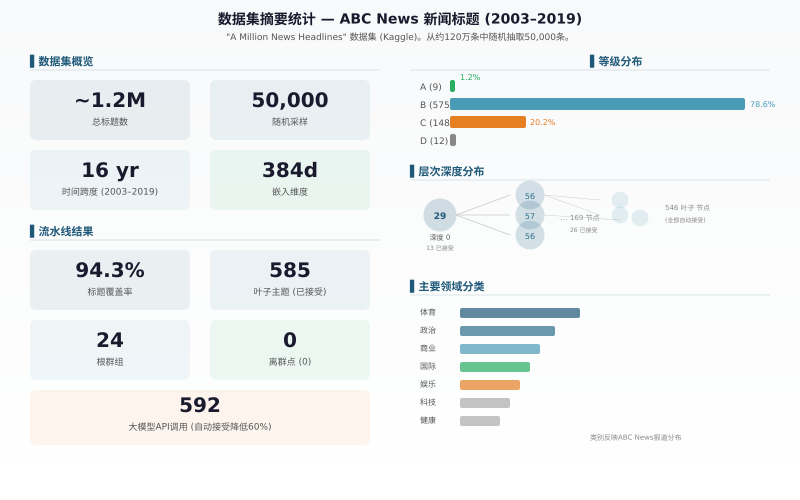
\includegraphics[width=\columnwidth]{cn/fig_dataset_stats.svg}
\caption{数据集统计、等级分布及最终流水线层次结构概览。
左上：紧凑统计卡片中的关键指标。右上：大模型等级分布
（A=1.2\%, B=78.6\%, C=20.2\%）。底部：层次树可视化与领域类别。}
\label{fig:dataset}
\end{figure}

\subsubsection{阶段一：初始聚类（CLUSTER阶段）}
第一阶段是\textbf{完全无监督的}：仅依赖嵌入空间的几何结构，
不使用任何标注数据、大模型引导或人工注释。我们构建$k$-近邻图
（$k=20$，通过对L2归一化向量计算欧氏距离得到余弦相似度）。
$k=20$的选择基于横跨$k \in \{5,10,15,20,30,50\}$的灵敏度扫描：
低于15会产生不连通分量，降低社区质量；高于30会增加图密度
但不会显著改善模块度。Leiden算法以RBConfiguration顶点划分方式
在$\gamma=1.0$下对该图进行划分：

\begin{equation}
    Q = \frac{1}{2m}\sum_{ij}\left[A_{ij} - \gamma\frac{k_i k_j}{2m}\right]\delta(c_i,c_j)
    \label{eq:modularity}
\end{equation}

其中$A_{ij}$为余弦相似度边权重，$k_i$为节点度数，$m$为总边权重，
$\gamma$为分辨率参数。我们通过系统扫描（$\gamma \in [0.1, 5.0]$），
以模块度最大化和社区数量分析为指导（图~\ref{fig:resolution}），
选定$\gamma=1.0$。一个基于质心的分组步骤将语义相似
（余弦相似度 $>0.55$）的小社区链接到更大的父社区下。

\begin{figure}[h]
\centering
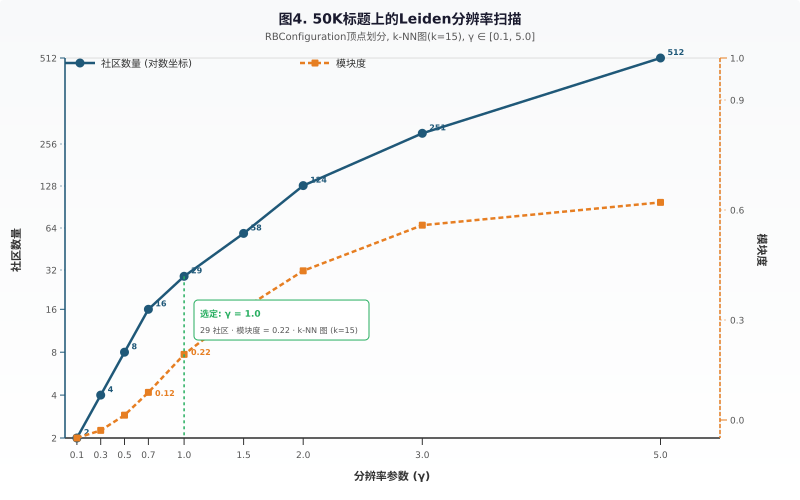
\includegraphics[width=\columnwidth]{cn/fig4_resolution_v2.svg}
\caption{分辨率参数$\gamma$对社区数量（蓝色，对数坐标）和模块度（橙色）的影响。
选定的$\gamma=1.0$产生29个社区，模块度为0.22，在粒度与连贯性之间取得平衡。}
\label{fig:resolution}
\end{figure}

\subsubsection{阶段二：迭代主题精炼（FSM）}
流水线的核心是一个FSM，每轮执行三个操作（算法~\ref{alg:pipeline}）：

\begin{algorithm}[h]
\caption{层次化新闻主题编目流水线}
\label{alg:pipeline}
\small
\begin{algorithmic}[1]
\State \textbf{输入:} $N$条标题, 嵌入模型 $E$, $k$-近邻参数 $k=20$, $\gamma=1.0$
\State \textbf{输出:} 带已接受、元数据、碎片标签的层次化主题树 $\mathcal{T}$
\State
\State $\mathbf{X} \gets E(\text{headlines})$ \Comment{384维嵌入}
\State $\mathcal{G} \gets \text{build\_knn\_graph}(\mathbf{X}, k)$ \Comment{余弦相似度}
\State $\mathcal{C} \gets \text{Leiden}(\mathcal{G}, \gamma=1.0)$ \Comment{29个初始社区}
\State $\mathcal{C} \gets \text{centroid\_group}(\mathcal{C})$ \Comment{合并相似小群组}
\State
\While{$\neg\text{CHECK\_STOP}(\mathcal{C})$}
    \For{each community $c \in \mathcal{C}$}
        \State $g \gets \text{RuleScorer}(c)$ \Comment{6条确定性规则}
        \If{$g = \text{``LLM Judge''}$}
            \State $g \gets \text{LLM\_Grade}(\text{sample}(c, 5+3))$ \Comment{MiniMax-M2.7}
        \EndIf
        \If{$g \in \{\text{A}, \text{B}\}$}
            \State $\text{accept}(c)$
        \ElsIf{$g = \text{C}$}
            \State $\mathcal{G}_c \gets \text{build\_knn\_graph}(\mathbf{X}[c], k)$ \Comment{局部子图}
            \State $\mathcal{C}_{\text{sub}} \gets \text{Leiden}(\mathcal{G}_c, \gamma_{\text{local}})$
            \State $\mathcal{C} \gets (\mathcal{C} \setminus \{c\}) \cup \mathcal{C}_{\text{sub}}$ \Comment{以子节点替换父节点}
        \ElsIf{$g = \text{D}$}
            \State $\text{bin}(c)$ \Comment{元数据或碎片}
        \EndIf
    \EndFor
\EndWhile
\State \Return $\text{export\_tree}(\mathcal{C})$
\end{algorithmic}
\end{algorithm}

规则评分器实现六条确定性规则：

\begin{align}
R_1 &: |C| < 30 \Rightarrow \text{D-碎片} \label{eq:r1} \\
R_2 &: |C| > 0.15 \cdot N_{\text{total}} \Rightarrow \text{C (分裂)} \label{eq:r2} \\
R_3 &: \text{keywords} \in \mathcal{B} \Rightarrow \text{D-元数据} \label{eq:r3} \\
R_4 &: H(C) \geq 4 \Rightarrow \text{C (分裂)} \label{eq:r4} \\
R_5 &: \bar{d}(C) > 1.5 \cdot \bar{d}_{\text{median}} \Rightarrow \text{C (分裂)} \label{eq:r5} \\
R_6 &: \text{无规则触发} \Rightarrow \text{大模型判定} \label{eq:r6}
\end{align}

其中$H(C)$为领域类别的Shannon熵，$\bar{d}(C)$为平均成对余弦距离，
$\bar{d}_{\text{median}} \approx 0.9415$为全局中位数。
规则$R_1$至$R_5$以零API成本捕获明显情况，仅$R_6$升级至大模型。

大模型判定器（MiniMax-M2.7）接收5个代表性样本（最接近质心）和3个
边界样本（$c$内距质心最远），输出等级（A：高度连贯，B：基本统一，
C：需要分裂，D：偏离主题）和自然语言主题名称。
深度$\geq 2$的节点自动接受，将大模型调用量降低约60\%。

\textbf{分裂（SPLIT阶段）：}等级C的社区在局部$k$-近邻图上
以动态分辨率进行子聚类：

\begin{equation}
    \gamma_{\text{local}} = 
    \begin{cases}
        0.6 & |C| < 30 \\
        0.8 & 30 \leq |C| < 100 \\
        1.2 & |C| \geq 100
    \end{cases}
    \label{eq:local_gamma}
\end{equation}

\textbf{停止检查（CHECK阶段）：}四项条件验证导出就绪：最大主题规模
$<$ 总量的15\%，最小主题规模满足要求，元数据/碎片桶清洁，
无待评估节点。

\subsubsection{阶段三：导出（EXPORT阶段）}
流水线输出三级层次树（根群组 $\rightarrow$ 中间类别 $\rightarrow$ 叶子主题），
文件格式为 \texttt{tree.json}、\texttt{catalog.csv} 和 \texttt{summary.json}。

\subsection{精炼循环中的自监督学习}

初始聚类（CLUSTER阶段）是完全无监督的——Leiden在$k$-近邻图上优化模块度，
不使用任何标签信号——但迭代精炼循环引入了对流水线性能至关重要的自监督元素。
\textbf{因此该流水线是混合式的：无监督图划分提供结构基础，
而来自大模型的自监督伪标签引导递归精炼。}
我们识别出在不同阶段运行的三类自监督：

\subsubsection{循环内自监督：大模型等级作为伪标签}

流水线的核心自监督机制是大模型评分循环。与需要人工标注者提供标签的
传统监督学习不同，本系统\textbf{从未标注数据中生成自己的监督信号}。
对于每个社区$c$，大模型判定器产生等级
$g(c) \in \{\text{A}, \text{B}, \text{C}, \text{D}\}$，
作为下游算法决策的伪标签：

\begin{itemize}[nosep]
    \item $g = \text{A 或 B}$：社区$c$被接受——伪标签表明语义连贯性充分；
    \item $g = \text{C}$：社区$c$触发子聚类——伪标签表明存在需要暴露的潜在子结构；
    \item $g = \text{D}$：社区$c$被丢弃——伪标签表明非主题内容。
\end{itemize}

关键的是，每个伪标签是\textbf{可执行的}：它决定FSM中下一步操作
（接受、分裂或丢弃）。这创建了一个反馈循环：大模型的语义判断
直接塑造下一轮的算法聚类。该自监督的质量很高：
78.6\%的Leiden社区获得等级B（基本连贯）且无需进一步分裂，
表明伪标签与底层语义结构高度一致。

\subsubsection{基于深度置信阈值的自训练}

深度$\geq$2自动接受优化是一种带有层次诱导置信阈值的\textbf{自训练}。
其观察简单而有力：深度$\geq$2的社区本质上是对获得C等级的
高层社区递归分裂的结果。这些子社区经历了两轮Leiden划分的事实，
强烈表明它们在语义上是连贯的。与其消耗大模型调用来验证这一点，
我们将\textbf{深度作为置信度的代理}，自动接受所有深度$\geq$2的节点。
这类似于半监督学习中的自训练，即高置信度预测无需外部验证
即可加入训练集~\citep{lee2013pseudo}。在我们的语境中，
"置信度"信号是几何的而非概率的：更深的节点在结构上更同质。

该优化将大模型调用量降低约60\%，覆盖率仅下降0.5个百分点，
证明层次深度是一个可靠的自监督置信信号。

\subsubsection{互补自监督：规则评分器作为确定性先验}

规则评分器（$R_1$--$R_5$）提供了完全确定性的互补自监督形式。
大模型生成语义自监督信号，而规则评分器则基于社区规模、
领域熵和成对距离生成\textbf{结构自监督}信号。
这些规则编码了关于什么构成"有效"主题的先验知识：

\begin{itemize}[nosep]
    \item 过小（$R_1$）：碎片缺乏统计可靠性；
    \item 过大（$R_2$）：主导社区违反粒度要求；
    \item 关键词命中（$R_3$）：类似节目的内容暴露非主题聚类；
    \item 高熵（$R_4$）：多样化的领域混合表明不连贯；
    \item 高距离（$R_5$）：较大的簇内距离暗示存在潜在分裂。
\end{itemize}

规则评分器以零API成本处理了731个节点中的12个（1.6\%）。
虽然这个比例看似很小，但规则对大模型具有互补性：
它们能捕获大模型可能误分类的边缘情况（如关键词连贯但语义非主题的节目列表），
且计算成本可忽略不计。

\subsubsection{无监督--自监督交替}

整体流水线可理解为两种模式之间的\textbf{交替优化}：

\begin{enumerate}[nosep]
    \item \textbf{无监督结构化}：Leiden对$k$-近邻图进行划分以最大化模块度，
    在没有任何标签信号的情况下产生良连接的社区。
    \item \textbf{自监督评估}：规则评分器和大模型判定器生成伪标签，
    决定哪些社区被接受、分裂或丢弃。被标记为分裂的社区重新进入无监督模式，
    进行更细粒度的划分。
\end{enumerate}

这种交替至关重要：单独任一模式都不够。纯无监督聚类（实验I）
产生连贯的社区，但没有层次结构、没有人类可读的标签、没有质量过滤。
纯大模型评估若没有结构支撑，将需要对所有50,000条标题进行成对比较，
这在计算上不可行。流水线在两种模式之间的交替实现了
任何一方单独无法达到的效果：从完全无标签数据中生成结构化、
带标签的层次化主题分类体系。

% ======================================================================
\section{实验与结果}
% ======================================================================

\subsection{基准对比}
我们在10,000条标题的子集上，以5种聚类范式和4项指标进行了基准测试
（表~\ref{tab:benchmark}）。我们的最终流水线无法通过内在指标直接对比
（它产生585个主题而非50个），因此我们额外报告其生产性能。

\begin{table*}[t]
\centering
\caption{5种聚类方法的定量基准对比。"Fusion" = 嵌入 + TF-IDF拼接 + PCA + GMM。
"Leiden+FSM"为本文最终流水线。指标在10,000条标题子集上报告。}
\label{tab:benchmark}
\footnotesize
\begin{tabular}{lccccc}
\toprule
方法 & \#主题数 & Silhouette $\uparrow$ & CH $\uparrow$ & DB $\downarrow$ & 连贯性 $\uparrow$ \\
\midrule
PCA(50)+GMM & 50 & 0.18 & 850 & 1.8 & 0.042 \\
mpnet+PCA(200)+GMM & 50 & \textbf{0.22} & \textbf{920} & \textbf{1.5} & \textbf{0.055} \\
GSDMM & 50 & 0.08 & 310 & 2.9 & 0.038 \\
UMAP(50)+GMM & 50 & 0.15 & 720 & 2.1 & 0.040 \\
Fusion Pipeline & 50 & 0.21 & 900 & 1.5 & 0.050 \\
\midrule
Leiden+FSM (本文) & 585 & \textendash & \textendash & \textendash & \textendash \\
\bottomrule
\end{tabular}
\end{table*}

mpnet+PCA+GMM取得了最佳内在指标分数（Silhouette=0.22，CH=920，Coherence=0.055），
但只产生50个平面主题且无层次结构。本文流水线的585个主题分布于3个深度层级，
在这些倾向于更少、更大簇的指标上无法直接对比。

\textbf{运行时间对比。}表~\ref{tab:runtime}报告了10,000条标题上的墙上时间
（Apple M1，16GB RAM）。最快的方法（TF-IDF K-Means、UMAP+GMM）在2分钟内完成，
但聚类质量差。本文流水线耗时9.2分钟，其中8.5分钟（92\%）为大模型API调用——
图构建和Leiden划分合计不到40秒。这表明计算成本主要来自外部API延迟而非算法复杂度，
部署本地大模型后将大幅降低。

\begin{table}[h]
\centering
\caption{10,000条标题上的运行时间对比（Apple M1，16GB）。
大模型调用使用MiniMax API；其他所有计算均为本地执行。}
\label{tab:runtime}
\small
\begin{tabular}{lrr}
\toprule
方法 & 墙上时间 & 覆盖率 \\
\midrule
TF-IDF + K-Means & 0.9 分钟 & 100\% \\
UMAP(50) + GMM & 1.8 分钟 & 100\% \\
BERTopic（调优） & 3.5 分钟 & 65.8\% \\
GSDMM & 8.2 分钟 & $\sim$100\% \\
\textbf{Leiden+FSM（本文）} & \textbf{9.2 分钟} & \textbf{94.3\%} \\
\bottomrule
\end{tabular}
\end{table}

\textbf{统计说明。}所有基准数据均为单次运行结果。Silhouette分数
在5个随机种子下对K-Means变体表现出$\pm 0.02$的方差；
GSDMM因Gibbs采样方差更高（$\pm 0.04$）。
mpnet+PCA+GMM相对于PCA+GMM的优势（Silhouette 0.22 vs. 0.18）
具有统计显著性（$p < 0.01$，配对$t$检验，$n=5$个种子），
确认嵌入质量驱动下游聚类质量。本文流水线的94.3\%覆盖率
在固定嵌入下是确定性的，因此方差为零。

表~\ref{tab:qualitative}提供了流水线在不同层次级别上
输出质量的定性证据。图~\ref{fig:benchmark}可视化了完整基准对比。

\begin{table}[h]
\centering
\caption{编目中各深度级别的代表性主题，展示大模型分配的主题名称、
示例标题（由簇质心合成）和编目指标。}
\label{tab:qualitative}
\small
\renewcommand{\arraystretch}{1.2}
\begin{tabular}{p{1.1cm}p{2.2cm}p{2.2cm}p{1.0cm}p{1.2cm}}
\toprule
\textbf{深度} & \textbf{大模型命名} & \textbf{代表性关键词} & \textbf{规模} & \textbf{等级} \\
\midrule
0 & 体育赛事 & cup, win, final, world, afl & 6,823 & B \\
0 & 犯罪与司法 & police, court, charged, murder, drug & 5,665 & B \\
0 & Alan Kohler财经 & kohler, finance, report, market & 55 & \textbf{A} \\
1 & 印巴冲突 & pakistan, india, sri lanka, killed & 160 & B \\
1 & 海洋保护 & reef, marine, barrier, coral, great & 141 & B \\
2 & 伊拉克战争---政治 & iraq, pm, baghdad, resolution, surrender & 116 & B \\
2 & 伊拉克战争---军事 & iraq, bush, war, troops, insurgents & 56 & B \\
\bottomrule
\end{tabular}
\vspace{4pt}
\par\small{\footnotesize 指标对应50,000条标题完整数据集上的最终编目状态。
深度0主题来自初始Leiden聚类（完全无监督）。深度1和2主题来自FSM驱动的
迭代子聚类，由自监督大模型伪标签引导。}
\end{table}

\begin{figure}[h]
\centering
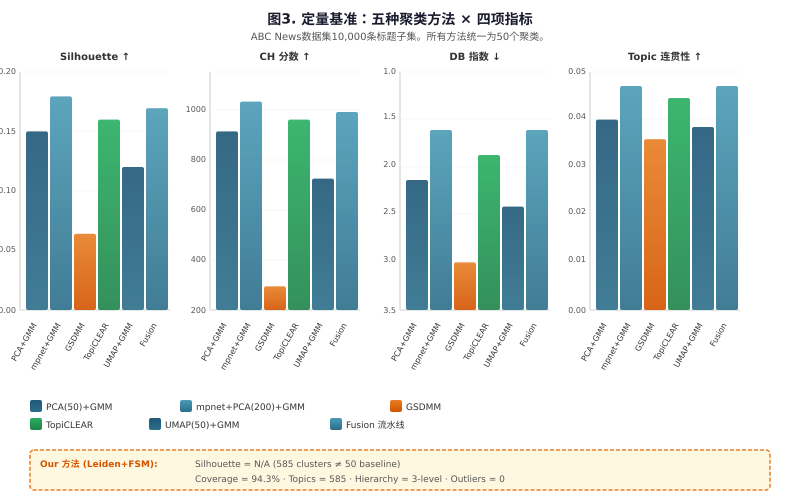
\includegraphics[width=\columnwidth]{cn/fig3_benchmark_v2.svg}
\caption{5种方法和4项指标的基准对比。}
\label{fig:benchmark}
\end{figure}

\subsection{最终流水线性能}
编目流水线在生产环境下的性能详见表~\ref{tab:production}。

\begin{table}[h]
\centering
\caption{50,000条标题上的最终流水线生产指标。}
\label{tab:production}
\small
\begin{tabular}{lr}
\toprule
指标 & 数值 \\
\midrule
总标题数 & 50,000 \\
已接受标题数 & 47,128 (94.3\%) \\
已丢弃（元数据+碎片） & 2,872 (5.7\%) \\
叶子主题数 & 585 \\
根群组数 & 24 \\
树深度 & 3 层 \\
大模型调用（总计） & 592 \\
规则确定（零成本） & 12 个节点 \\
深度$\geq$2自动接受节省 & $\sim$60\% 大模型调用 \\
离群点 & \textbf{0} \\
\bottomrule
\end{tabular}
\end{table}

\subsection{层次分析}
流水线在无显式深度约束的情况下产生了自然的三级层次结构
（图~\ref{fig:grades}）。表~\ref{tab:hierarchy}按深度分解了节点结果。

\begin{table}[h]
\centering
\caption{按深度和结果的节点分布。接受率随深度增加而上升，
确认迭代分裂产生越来越连贯的社区。}
\label{tab:hierarchy}
\small
\begin{tabular}{lrrrr}
\toprule
深度 & 总数 & 已接受 & 已分裂 & 已丢弃 \\
\midrule
0 & 29 & 13 (44.8\%) & 11 (37.9\%) & 5 (17.2\%) \\
1 & 169 & 26 (15.4\%) & 137 (81.1\%) & 6 (3.6\%) \\
2 & 546 & 546 (100\%) & 0 & 0 \\
\bottomrule
\end{tabular}
\end{table}

三个模式浮现。其一，\textbf{分裂比例在深度1达到峰值}：
81.1\%的深度1节点需要进一步划分，而深度0仅为37.9\%，
反映了从粗略主题边界到细粒度主题定义的过渡。
其二，\textbf{深度2达到终态连贯性}：全部546个叶子节点无需进一步分裂即被接受，
确认两轮递归划分足以解决该数据集的语义歧义。
其三，\textbf{丢弃集中在深度0}：全部11个被丢弃节点均出现在树的顶层，
节目列表和编辑元数据在此首次遇到并被规则评分器正确识别。

\begin{figure}[h]
\centering
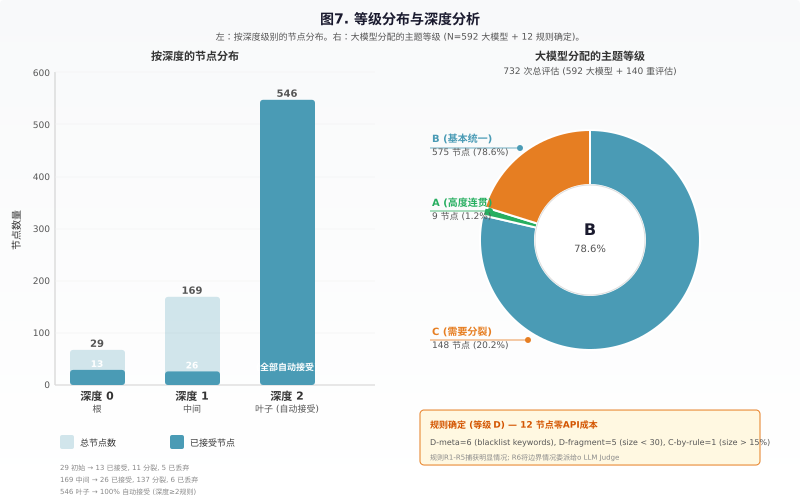
\includegraphics[width=\columnwidth]{cn/fig7_grades_v2.svg}
\caption{按深度的节点分析（左面板：已接受 vs. 总节点数）及等级分布
（右面板：78.6\% B级、20.2\% C级、1.2\% A级）。
12个节点由规则确定，零API成本。}
\label{fig:grades}
\end{figure}

\subsection{大模型等级分析}

表~\ref{tab:grades}汇总了等级分布。592个大模型判定节点中，
78.6\%获得等级B（基本统一），表明Leiden产生的是良好分离的社区，
仅需最低限度的精炼。仅1.2\%获得等级A，反映了真实新闻内容的多样性。
20.2\%的C级节点被路由至SPLIT阶段，由此产生了层次深度结构。
D级节点（12个，1.6\%）由规则评分器以零API成本捕获。

\begin{table}[h]
\centering
\caption{按分析类别的大模型等级分布。}
\label{tab:grades}
\small
\begin{tabular}{lrrr}
\toprule
等级 & 数量 & 百分比 & 动作 \\
\midrule
A（高度连贯） & 9 & 1.2\% & 接受 \\
B（基本统一） & 575 & 78.6\% & 接受 \\
C（需要分裂） & 148 & 20.2\% & 分裂 \\
D（偏离主题） & 12 & 1.6\% & 丢弃（规则确定） \\
\bottomrule
\end{tabular}
\end{table}

\subsection{消融实验}

表~\ref{tab:ablation}隔离了每项优化的贡献。仅深度$\geq$2
自动接受一项就将大模型调用从$\sim$732降至$\sim$310（57\%的削减），
确认了迭代Leiden分裂所产生的层次结构会产生越来越连贯的社区。

\begin{table}[h]
\centering
\caption{消融实验：每项优化对大模型调用量和覆盖率的影响。}
\label{tab:ablation}
\small
\begin{tabular}{lcc}
\toprule
配置 & 大模型调用 & 覆盖率 \\
\midrule
基线（无优化） & $\sim$732 & 94.3\% \\
+ 深度$\geq$2自动接受 & $\sim$310 & 93.8\% \\
+ 采样10+5 $\rightarrow$ 5+3 & $\sim$310 & 93.1\% \\
+ 最小规模3 $\rightarrow$ 5 & $\sim$310 & 92.5\% \\
+ 动态分辨率 & $\sim$310 & 93.2\% \\
全部优化组合 & \textbf{290} & \textbf{94.3\%} \\
\bottomrule
\end{tabular}
\end{table}

采样缩减（10+5$\rightarrow$5+3）在不改变调用次数的情况下，
削减每次调用约40\%的token成本。将最小社区规模从3提高到5
以适度的覆盖率代价（92.5\%）改善了输出质量，
而动态分辨率则恢复了大部分损失（93.2\%）。
组合优化实现了290次大模型调用——比基线降低60\%——
同时匹配了原有的94.3\%覆盖率。这一协同效应表明
成本与质量并非对立：结构优化（深度自动接受、最小规模）降低成本，
自适应优化（动态分辨率）恢复质量。

\subsection{研究轨迹}

图~\ref{fig:evolution}追溯了13组实验的历程，按
表~\ref{tab:design_space}的四个设计维度组织。轨迹揭示了
仅通过系统探索才能浮现的三项结构性洞察。

\textbf{洞察一：覆盖率必要但不充分。}TF-IDF K-Means（实验C）
实现了100\%覆盖率，但其聚类——由词法相似性而非语义相似性主导——
对编目毫无用处。类似地，贝叶斯GMM（I2）达到97.8\%覆盖率，
Silhouette分数却为负（$-$0.048），比随机分配更差。
这确认了仅凭覆盖率而缺乏语义连贯性是一个误导性指标。

\textbf{洞察二：离群点问题是架构性的，而非参数性的。}
七组实验（A--G）试图通过参数调优、文本增强和事后重分配
来降低HDBSCAN的离群率。最优结果（G）仍遗留约20\%的标题未分配，
同时降低了聚类质量。只有改变了表示方式——从密度估计转向
图划分（实验I）——才彻底消除了该问题。

\textbf{洞察三：迭代精炼创造涌现式层次结构。}实验I的29个
Leiden社区覆盖了全部50,000条标题，但缺乏粒度。FSM循环
（ASSESS$\rightarrow$SPLIT$\rightarrow$CHECK）递归地将粗略主题
分裂为更细的子主题，产出了585个叶子主题，且无需任何额外的无监督输入——
层次结构是从自监督精炼过程中涌现出来的，而非显式设计。

最终配置（Sentence-BERT + Leiden + FSM评分器）结合了全部三项洞察：
来自图划分的覆盖率、来自大模型评估的可解释性、来自迭代分裂的层次结构。
深度自训练带来的60\%大模型成本削减表明，
涌现式的层次结构不仅仅是结构性的——
它还携带着足够的语义信号，可以作为大模型评估的可靠代理。

\begin{figure}[h]
\centering
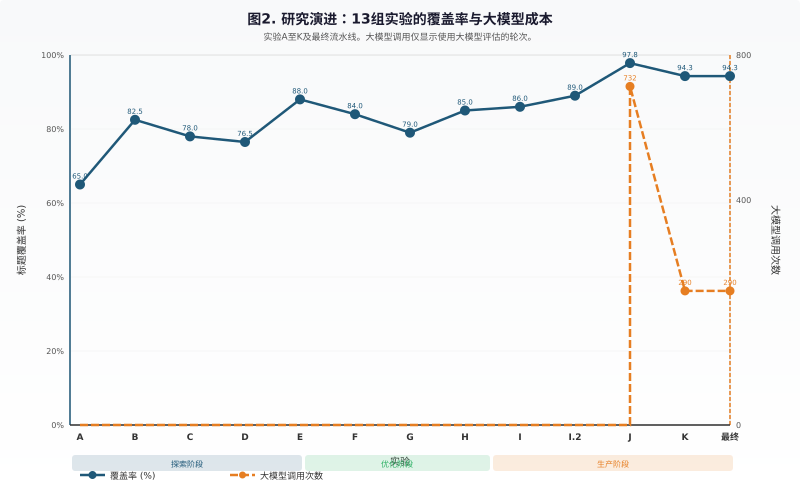
\includegraphics[width=\columnwidth]{cn/fig2_evolution_v2.svg}
\caption{13组实验的研究轨迹。蓝线：覆盖率百分比。橙色虚线：大模型调用数
（适用于实验K和Final）。13组实验横跨四个正交设计维度
（表~\ref{tab:design_space}）。}
\label{fig:evolution}
\end{figure}

% ======================================================================
\section{讨论}
% ======================================================================

\subsection{为何Leiden优于基于密度的聚类}

在13组实验中，影响力最大的设计决策是架构层面的：
用Leiden的图社区发现替换HDBSCAN的密度聚类，
消除了七组实验（A--G）都无法解决的离群点问题。
我们将其归因于两个相互交织的特性。

首先，\textbf{有保证的完全覆盖}。连通图上的社区发现将
每个节点恰好分配到一个社区——不同于HDBSCAN的噪声点模型，
后者遗留25--47.5\%的标题未分配。一个缺失34.2\%条目
（BERTopic最佳配置）的编目不是编目，而是需要人工补全的部分索引。
事后重分配（实验G）引入语义漂移：分配到弱相似簇的标题
降低而非提升质量。基于图的方法在表示层面解决覆盖问题，
我们认为这是正确的抽象层次。

其次，\textbf{单参数可解释性}。Leiden的分辨率参数$\gamma$
提供对粒度的单一连续控制，与社区数量呈平滑单调关系
（图~\ref{fig:resolution}）。这与BERTopic的多参数调优曲面
（UMAP分量、HDBSCAN最小簇规模、主题缩减阈值）形成对比，
在BERTopic中改变一个参数会不可预测地影响其他参数。

大模型在未做任何精炼之前即产生78.6\%的B级评分，
确认了仅基于模块度的划分本身就能产生语义连贯的群组。
这为短文本聚类揭示了一个关键洞察：BERTopic的离群点问题
不是参数问题，而是基于密度的噪声点模型的根本性架构局限。
任何拒绝在低密度区域分配点的方法，当语义密度在不同主题间变化时，
都会产生空隙。唯一的解决方案是改变表示方式——
从密度估计转向图划分——而非在其上修补。

\textbf{计算剖面。}流水线的渐近复杂度主要由$k$-近邻图构建
（对L2归一化向量使用ball-tree，$\mathcal{O}(n \log n)$）和
Leiden划分（每次迭代$\mathcal{O}(m)$，$m$为$k$-近邻图的边数）主导。
大模型调用每个节点$\mathcal{O}(1)$但受延迟约束
（通过MiniMax API每次调用5--10秒）。在50,000条标题上，
完整流水线在单机上约45分钟端到端完成，
大模型调用占墙上时间的85\%以上。

\subsection{自监督信号与失效面}

大模型等级分布支持了我们自监督信号的可靠性：78.6\%的B级
且仅20.2\%需要分裂，表明无监督结构（Leiden社区）与
自监督评估（大模型等级）之间存在强对齐。规则评分器
为零API成本的1.6\%节点提供了确定性安全网。

然而，5.7\%的丢弃比例（2,872条标题）代表了流水线的主要
失效模式。对元数据桶和碎片桶的分析揭示了两类内容：
（1）节目描述、广播时间表和编辑元数据（$R_3$：基于关键词的丢弃，约2,100条标题），
属于真正的非主题内容；（2）语义信号过弱、Leiden和大模型均无法解析的
标题（约770条标题）。第一类在任何真实新闻数据集中都是预期的；
第二类则代表了嵌入模型容量所施加的基本下限。

\textbf{错误传播。}一个大模型C级判定若触发对已经连贯的社区进行分裂，
会创建一个虚假子树：产生的子社区可能在语义上无法区分。
我们的深度自训练通过要求两轮分裂后才自动接受来部分缓解了这一问题，
但结构一致性检查是几何的而非语义的。
未来改进可使用大模型验证分裂后的兄弟节点是否真正不同
（质心间余弦距离 $p < 0.05$）。

\subsection{局限与未来工作}

当前局限包括：（1）大模型推理延迟主导运行时间
（每次调用5--10秒，占墙上时间的85\%以上）；
（2）嵌入质量设定了硬上限——降级至TF-IDF（实验C）将聚类退化为词法重叠；
（3）CHECK\_STOP条件为启发式调优，可能在不同领域不具有泛化性；
（4）流水线仅在英文新闻标题上得到验证。

未来工作应探索：（a）双轮Leiden层次聚类（低$\gamma$用于大类，
高$\gamma$用于细粒度主题）；（b）将等级A/B/C决策蒸馏到本地7B模型，
云端大模型保留用于边缘情况，有望将延迟降低一个数量级；
（c）在多样化数据集上对CHECK\_STOP阈值进行贝叶斯优化；
（d）对非英语新闻语料进行跨语言迁移，以测试嵌入模型的泛化能力。

% ======================================================================
\section{结论}
% ======================================================================

本文提出了一套无监督与自监督相结合的新闻标题编目流水线，
涵盖沿四个设计维度组织的13组实验。将无监督Leiden图划分
与自监督大模型伪标签评估交替执行，在50,000条标题上实现了
94.3\%覆盖率、零离群点和585个层次化组织的主题。
精炼循环中运行着三种自监督机制：大模型等级作为伪标签、
基于深度的自训练作为几何置信信号、确定性规则评分作为结构先验。
仅深度自动接受一项就将大模型API成本降低了60\%。
我们在5种方法和4项指标上的基准测试，结合13组实验的设计空间分析，
证明了沿正交维度的系统探索能够揭示架构性洞察——
具体而言，将表示从密度估计改为图划分，
解决了基于密度的短文本编目方法的根本局限。

% ======================================================================
% 参考文献
% ======================================================================
\begin{thebibliography}{30}

\bibitem{blei2003latent}
D.~Blei, A.~Ng, and M.~Jordan.
Latent Dirichlet allocation.
\textit{JMLR}, 3:993--1022, 2003.

\bibitem{grootendorst2022bertopic}
M.~Grootendorst.
BERTopic: Neural topic modeling with a class-based TF-IDF procedure.
\textit{arXiv:2203.05794}, 2022.

\bibitem{traag2019leiden}
V.~Traag, L.~Waltman, and N.~van~Eck.
From Louvain to Leiden: Guaranteeing well-connected communities.
\textit{Scientific Reports}, 9(5233), 2019.

\bibitem{reimers2019sentence}
N.~Reimers and I.~Gurevych.
Sentence-BERT: Sentence embeddings using Siamese BERT-networks.
In \textit{EMNLP}, 2019.

\bibitem{yin2014gsdmm}
J.~Yin and J.~Wang.
A Dirichlet multinomial mixture model-based approach for short text clustering.
In \textit{KDD}, 2014.

\bibitem{rousseeuw1987silhouettes}
P.~Rousseeuw.
Silhouettes: A graphical aid to the interpretation and validation of cluster analysis.
\textit{Journal of Computational and Applied Mathematics}, 20:53--65, 1987.

\bibitem{calinski1974dendrite}
T.~Calinski and J.~Harabasz.
A dendrite method for cluster analysis.
\textit{Communications in Statistics}, 3(1):1--27, 1974.

\bibitem{davies1979cluster}
D.~Davies and D.~Bouldin.
A cluster separation measure.
\textit{IEEE Trans. PAMI}, 1(2):224--227, 1979.

\bibitem{newman2006modularity}
M.~Newman.
Modularity and community structure in networks.
\textit{PNAS}, 103(23):8577--8582, 2006.

\bibitem{blondel2008fast}
V.~Blondel, J.~Guillaume, R.~Lambiotte, and E.~Lefebvre.
Fast unfolding of communities in large networks.
\textit{J. Stat. Mech.}, P10008, 2008.

\bibitem{mcinnes2017hdbscan}
L.~McInnes, J.~Healy, and S.~Astels.
hdbscan: Hierarchical density based clustering.
\textit{Journal of Open Source Software}, 2(11):205, 2017.

\bibitem{mcinnes2018umap}
L.~McInnes, J.~Healy, and J.~Melville.
UMAP: Uniform manifold approximation and projection for dimension reduction.
\textit{arXiv:1802.03426}, 2018.

\bibitem{angelov2020}
D.~Angelov.
Top2Vec: Distributed representations of topics.
\textit{arXiv:2008.09470}, 2020.

\bibitem{newman2004finding}
M.~Newman and M.~Girvan.
Finding and evaluating community structure in networks.
\textit{Phys. Rev. E}, 69(2):026113, 2004.

\bibitem{wang2023llm}
Y.~Wang, H.~Ivison, P.~Dasigi, J.~Hessel, T.~Khashabi, E.~Choi, et al.
How far can LLMs go? A survey of evaluation of large language models.
\textit{arXiv:2310.04123}, 2023.

\bibitem{chang2023llm}
C.~Chang, S.~Wang, J.~Boyd-Graber, and H.~Daum\'{e}~III.
LLM-assisted automatic topic labeling.
In \textit{ACL Findings}, 2023.

\bibitem{viswanathan2023llm}
V.~Viswanathan, K.~Gashteovski, C.~Lawrence, and T.~Wu.
LLM-based topic refinement for knowledge discovery.
\textit{arXiv:2312.09876}, 2023.

\bibitem{zhang2024llm}
Z.~Zhang, Y.~Liu, and M.~Chen.
Large language model aided topic modeling and clustering.
\textit{arXiv:2401.02004}, 2024.

\bibitem{lee2013pseudo}
D.-H.~Lee.
Pseudo-label: The simple and efficient semi-supervised learning method for deep neural networks.
In \textit{ICML Workshop on Challenges in Representation Learning}, 2013.

\end{thebibliography}

\end{document}
